\section{Contextualização}
O estado atual da comunicação mundial permite as pessoas, de qualquer país, comunicar e trocar conhecimento dos mais diversos assuntos. Essa facilidade de comunicação também facilita a união de indivíduos, que não se conhecem e com realidades sociais completamente opostas, em um projeto com metas em comum.

Um exemplo, dessa união incomum, é o caso de um carpinteiro sul-africano que, ao perder os dedos numa serra, e ficar insatisfeito com os preços e qualidade das próteses disponíveis no mercado, resolveu iniciar um projeto open source de mão biônica com a ajuda de um técnico de efeitos especiais que mora nos EUA. Juntos, esses dois indíviduos que até então não se conheciam, conseguiram criar um projeto de mão biônica por 150 dólares. Após isso, o projeto ganhou visibilidade e patrocínio e já está sendo testado por algumas crianças deficientes da africa do sul\footnote{\label{maobionica} Notícia sobre projeto de mão biônica \url{http://meiobit.com/115807/}}.

Essa melhoria de comunicação, obviamente, também  afeta o campo empresarial. Em algumas empresas, o sistema de "Outsourcing", que é um sistema de aquisição de conhecimento ou tecnologia, começou a ser substituído pelo sistema de "Crowndsourcing", que no campo empresarial, funciona como uma espécie de concorrência: a empresa lança uma espécie de edital informando quanto pode pagar por determinada solução e quem quer que seja poderá oferecer a resposta adequada ao que se procura, independente de ser uma, duas, ou cem pessoas, contanto que resolva o problema.

De modo geral Crowdsourcing é a prática de obtenção de serviços, idéias ou conteúdo solicitando contribuições de um grande grupo de pessoas e, especialmente, a partir de uma comunidade on-line, ao invés de funcionários ou fornecedores tradicionais \footnote{\label{wiki-crowd} Definição completa de crowdsourcing \url{ http://en.wikipedia.org/wiki/Crowdsourcing}}.
Existem diversos tipos de crowdsourcing, mas nesse trabalho iremos nos focar no crowdsourcing conhecido como \emph{Wisdom of the Crowd} que é um tipo de crowdsourcing que coleta grandes quantidades de informação e as agrega para obter uma visão completa e precisa sobre um determinado tema. Essa visão, dependendo do tema de estudo, pode ser representada por um mapa de crowdsourcing.

A produção de mapas crowdsourcing é geralmente feita de forma automática, usualmente temos algum software e/ou site que coleta as informações e as agrupa por meio de algum algorítimo desenvolvido especificamente para o mapa.

A coleta dessas informações pode ocorrer de várias formas, tanto manual como automática. Por exemplo, no site \citeauthoronline{portoalegre} os usuários podem adicionar novas informações através do site, ou seja, ela é feita de forma manual. Alguns sistemas podem coletar informações de forma automática usando programas de computadores, aplicativos de smartphones \cite{thiagarajan_cooperative_2010}  e até mesmo da internet\footnote{ Mapa com informações coletadas do Twitter \url{http://trendsmap.com}}.

Uma vez coletada, essa informação é analisada e exibida em um mapa, mas o mapa em si não é o produto final, e sim algumas informações específicas retiradas dele. Por exemplo, podemos ter mapas que mostrem os congestionamentos no trânsito de uma cidade e um sistema \cite{thiagarajan_vtrack:_2009} que através desse mapa consegue identificar  uma rota mais eficiente com menor consumo de energia, evitando assim ficar parado no congestionamento gastando gasolina.

Em alguns casos, mapas de crowdsourcing possuem informações posicionadas em regiões muito próximas entre si, que devido a quantidade elevada, acabam poluindo a visualização e dificultando a compreensão do mapa. Esse problema pode ser resolvido quando os mapas oferecem mecanismos para agrupar e filtrar essas informações. Um mecanismo ideal é o zoom contextual ou zoom em grupo, que filtra informações irrelevantes, em determinados níveis de zoom, deixando o mapa mais leve e compreensível.

O Projeto Searchlight pretende ser uma ferramenta para auxiliar e melhorar a visualização de mapas de crowdsourcing.

O escopo do projeto atinge a criação de uma ferramenta que visualize mapas de crowdsourcing em um navegador de internet, tanto desktop quanto mobile, usando recursos de visualização de mapas já disponíveis em HTML5 mas que ainda não possuem zoom contextual e outras opções úteis que permitam uma melhor visualização do mapa.



\section{Definição do Problema}
Mapas de crowdsourcing tendem a mostrar uma enorme quantidade de informação. Essa característica faz com que, em alguns casos, a visualização e a compreensão do mapa seja comprometida.
 
Ao trabalhar com mapas de crowdsourcing, geralmente encontramos 2 problemas: a sobreposição de informações e o zoom arbitrário. 



\subsection{Sobreposição de Informações}
O site \citeauthoronline{portoalegre} é um exemplo da importância do mapas de crowdsourcing no contexto governamental e na sociedade. Por meio desse site os cidadãos de porto alegre podem relatar os problemas de sua cidade para que as autoridades tomem as devidas providências. 

Um dos principais objetivos do site é identificar as áreas prioritárias em que o governo deveria atuar. Mas a sobreposição de informações dificulta essa tarefa, pois ocorre frequentemente nesse site. 

\begin{figure}[htb]
	\caption{\label{fig-porto-alegre} Sobreposição de informações no mapa do site PortoAlegre.cc}
	\begin{center}
	    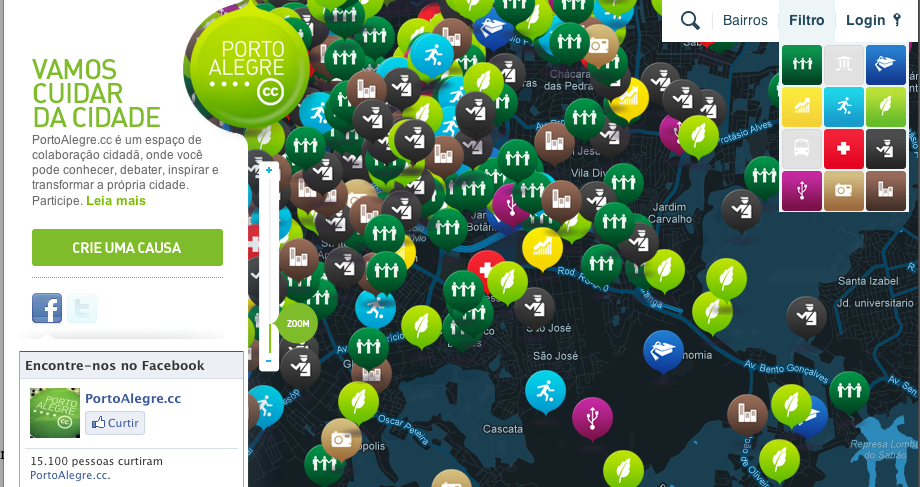
\includegraphics[scale=0.4]{portoalegre-cc}
	\end{center}
	\legend{Fonte: \citeonline{portoalegre}}
\end{figure}

Esse problema fica evidente na \autoref{fig-porto-alegre} quando consideramos, a possibilidade, que um grupo de 5 marcadores reunidos numa região específica, podem sobrepor dezenas ou até milhares de outros marcadores. Ou seja, o mapa não consegue mostrar, com clareza e precisão, as áreas de maior ocorrência de determinado incidente. 

O site fornece um filtro por categorias, que diminui de forma significativa a quantidade de informação exibida.  Mas infelizmente não resolve o problema, pois a sobreposição de informação ainda pode ocorrer com informações de uma mesma categoria.





\subsection{Zoom arbitrário}
Alguns sites criam mecanismos que minimizam o problema da sobreposição de informações. Como exemplo, temos o \citeonline{crimemapatl}  mostrado na \autoref{fig-mapatl} que mostra um mapa com a taxa de crimes em Atlanta. 

O site fornece filtros por categoria, data e zoom. Mas o principal responsável pela eliminação da sobreposição de informação é o filtro por zoom. Esse filtro agrupa todos os marcadores que estão sobrepostos, no zoom atual, em um único marcador que exibe a informação somada dos marcadores que o compõem.
 
\begin{figure}[htb]
	\caption{\label{fig-mapatl} MapATL não possui sobreposição de informação devido ao filtro por zoom}
	\begin{center}
	    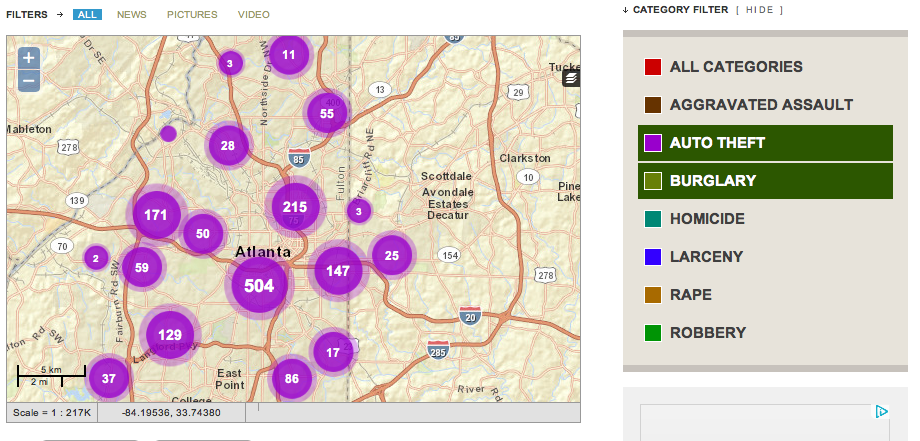
\includegraphics[scale=0.4]{crime-mapatl-com-filtro}
	\end{center}
	\legend{Fonte: \citeonline{crimemapatl}}
\end{figure}

Segundo \cite[42,44]{silva2010solap+} esse tipo de agrupamento, baseado em grelha, pode ser implementado a partir do algorítimo WaveCluster\cite{wavecluster}. 

 

\begin{figure}[htb]
	\caption{\label{fig-zoomab} Entre ZOOM A e ZOOM C existem muitos níveis intermediários e não apenas 1 (ZOOM B).}
	\begin{center}
	    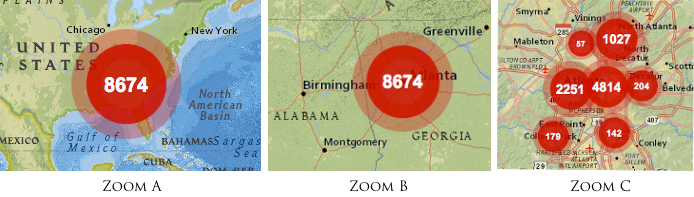
\includegraphics[scale=0.6]{zoomab}
	\end{center}
	\legend{Fonte: \citeonline{crimemapatl}}
\end{figure}

Esse algorítimo resolve o problema de sobreposição de informações. Porém o problema do zoom arbitrário, ilustrado na \autoref{fig-zoomab}, permanece.

O usuário precisa aplicar vários zoons para ir do ZOOM A para o ZOOM C. Mas durante essa interação é gasto tempo e banda, da conexão de internet, do usuário para exibir os zoons intermediários, quando o ideal seria exibir apenas o ZOOM B.

Esse gasto de banda, prejudica a usabilidade de mapas em dispositivos móveis pois, geralmente, eles possuem pouca banda de internet.

Uma abordagem para esse problema é o uso de um zoom inteligente que siga uma hierarquia espacial invés de simplesmente dobrar a visualização atual. 

\subsubsection{Informações arbitrárias}
Um subproblema do zoom arbitrário é a exibição de informações desnecessárias em todos os níveis de zoom. Na \autoref{fig-mapaufes} podemos observar o problema, que neste caso, a arbitrariedade está na exibição de informações, e não no número de zoons. 
 \begin{figure}[htb]
	\caption{\label{fig-mapaufes}Informações necessárias em níveis superiores, de zoom, visualizadas em níveis inferiores}
	\begin{center}
	    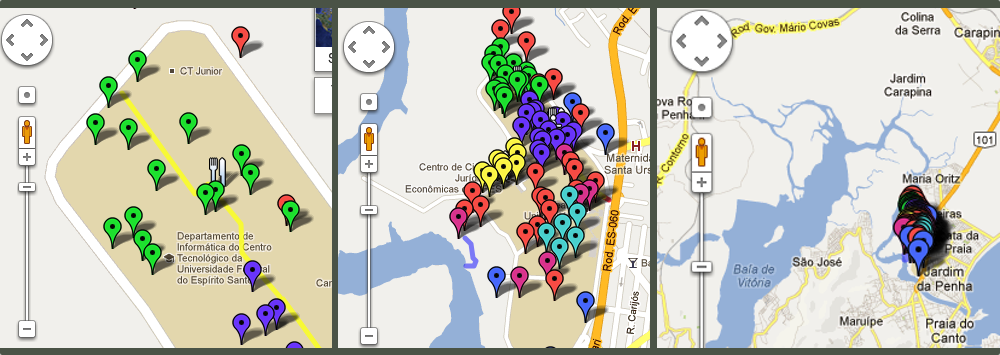
\includegraphics[scale=0.4]{ufes_map}
	\end{center}
	\legend{Fonte: http://maps.google.com}
\end{figure}
Os marcadores desse mapa exibem informações sobre os departamentos internos da UFES, mas essas informações são úteis apenas em certos níveis de zoom. Em níveis mais baixos, onde a área dessa universidade seja desprezível, a informação perde seu valor e fica poluindo o mapa. Neste caso, um único marcador representando o grupo seria mais útil.

\section{Objetivos}
Com base nas informações da definição do problema, o objetivo deste trabalho é desenvolver uma ferramenta que: agrupe marcadores de forma inteligente eliminando a sobreposição; forneça um zoom inteligente que não exiba níveis intermediários desnecessários; esconda marcadores quando sua informação não seja mais necessária ao nível observado.

O objetivo principal desse trabalho é facilitar a visualização de informação em mapas crowdsourcing. Isso devido a importância sócio-econômica das informações que geralmente são exibidas nessa classe de mapas. Mas a ferramenta poderia implementar recursos que também facilite a divulgação dessas informações. Por isso, o objetivo secundário é fornecer um mecanismo para gerar mapas a partir de planilhas de dados, e compartilhá-los sem que o autor precise programar ou ter algum conhecimento de programação. Para este trabalho a divulgação dos mapas é um objetivo secundário, mas poderia ser melhor abordado em trabalhos futuros.
  
\section{Contribuições}
A contribuição deste trabalho é o desenvolvimento de um framework para exibição de mapas em paginas web facilitando a visualização de informações crowdsourcing.

Além disso também foi criado um website do projeto\cite{gitsite} que explica e documenta o framework. O website fornece também um pagina de geração e compartilhamento de mapas por pessoas que não sabem programar.

\section{Estrutura da Monografia}
Este trabalho está organizado da seguinte forma:

Nesta introdução, é apresentado o contexto geral do projeto, a definição do problema, a solução proposta e a estrutura da monografia.

No capítulo 2, Fundamentação Teórica, apresenta-se uma explicação básica sobre os elementos comuns em mapas geográficos, usados na web, e suas relações com crowdsourcing; uma pesquisa sobre as estratégias para lidar com mapas que possuem muitos marcadores; uma pesquisa sobre algorítimos para agrupamento de pontos; uma revisão sobre o uso de planilhas eletrônicas como principal ambiente de programação para usuários finais em órgãos governamentais e seus usos como base de dados para informações geográficas.

No capítulo 3, Desenvolvimento, é explicado como o projeto foi desenvolvido, quais foram as ferramentas utilizadas, e o motivo da escolha de determinadas tecnologias. 

No capítulo 4, Solução Desenvolvida, é apresentado em detalhes a solução que foi desenvolvida e como utilizá-la.

No capitulo 5, Conclusão, é apresentado as dificuldades encontradas no decorrer do projeto, trabalhos futuros e conclusão geral sobre o projeto.



